% CVPR 2026 Paper Template; see https://github.com/cvpr-org/author-kit

\documentclass[10pt,twocolumn,letterpaper]{article}

%%%%%%%%% PAPER TYPE - UPDATE FOR FINAL VERSION
% \usepackage{cvpr}              % CAMERA-READY version
\usepackage[review]{cvpr}      % REVIEW version
% \usepackage[pagenumbers]{cvpr} % arXiv/page-number version

\usepackage{graphicx}
\usepackage{booktabs}
\usepackage{multirow}
\usepackage{amsmath}
\usepackage{amssymb}
\usepackage{xcolor}
\graphicspath{{figures/}}


\definecolor{cvprblue}{rgb}{0.21,0.49,0.74}
\usepackage[pagebackref,breaklinks,colorlinks,allcolors=cvprblue]{hyperref}

%%%%%%%%% PAPER ID - UPDATE IF NEEDED
\def\paperID{*****}
\def\confName{CVPR}
\def\confYear{2026}

\title{Video Super-Resolution with Classical Baselines, Temporal Propagation, and Adaptive Perceptual Fusion}

%%%%%%%%% AUTHORS - REPLACE WITH REAL GROUP INFORMATION
\author{Student 1\\
AIAA 3201 Introduction to Computer Vision\\
The Chinese University of Hong Kong, Shenzhen\\
{\tt\small student1@example.com}
\and
Student 2\\
AIAA 3201 Introduction to Computer Vision\\
The Chinese University of Hong Kong, Shenzhen\\
{\tt\small student2@example.com}
}

\begin{document}
\maketitle
\begin{abstract}
Video super-resolution (VSR) aims to reconstruct high-resolution videos from low-resolution inputs while preserving both spatial detail and temporal consistency. We implement a complete three-stage VSR pipeline following the project roadmap. Part~1 studies hand-crafted and early CNN baselines, including Bicubic, Lanczos, SRCNN, and simple temporal averaging. Part~2 reproduces modern pretrained super-resolution methods, including Real-ESRGAN, BasicVSR, and BasicVSR++. Part~3 proposes a lightweight adaptive hybrid refinement that fuses the temporally stable BasicVSR++ output with selected perceptual details from Real-ESRGAN using a pixel-wise uncertainty mask. We evaluate on mandatory REDS-sample, Vimeo, and real wild video data, and additionally run a full REDS validation benchmark over 30 sequences with PSNR, SSIM, LPIPS, FID, tLPIPS, qualitative rendering comparisons, zoom-in patches, and processed videos. On full REDS validation, BasicVSR++ achieves the best distortion fidelity with 31.7750 PSNR and 0.9016 SSIM, while the adaptive hybrid remains close at 31.6592 PSNR and 0.8987 SSIM with slightly lower LPIPS. GitHub repository: \url{https://github.com/Summer-916/AIAA3201-Video-Super-Resolution}.
\end{abstract}

\section{Introduction}
Video super-resolution reconstructs an HR video sequence from an LR observation. Unlike single-image super-resolution, VSR must recover fine image structures while also using temporal redundancy across neighboring frames. This makes the task a balance between spatial reconstruction, perceptual sharpness, and temporal stability. Classical interpolation methods are fast and stable but cannot hallucinate missing high-frequency details. Learned image SR methods such as SRCNN~\cite{dong2015srcnn}, SRGAN~\cite{ledig2017srgan}, and EDSR~\cite{lim2017edsr} improve spatial reconstruction, but frame-independent processing often ignores temporal coherence. Modern VSR models therefore introduce motion alignment and recurrent propagation, as represented by EDVR~\cite{wang2019edvr}, TDAN~\cite{tian2020tdan}, BasicVSR~\cite{chan2021basicvsr}, and BasicVSR++~\cite{chan2022basicvsrpp}.

This project implements and evaluates a practical VSR pipeline in three parts. First, we build classical and simple neural baselines to understand the behavior of interpolation, shallow CNN reconstruction, and naive temporal fusion. Second, we reproduce pretrained SOTA models: Real-ESRGAN~\cite{wang2021realesrgan} for perceptual enhancement and BasicVSR/BasicVSR++ for video-specific temporal propagation. Third, motivated by the fact that perceptual models can introduce hallucinated texture while distortion-oriented VSR can appear smooth, we design an adaptive hybrid method that combines the stable structure of BasicVSR++ with selected Real-ESRGAN details.

Our experiments cover the mandatory sample and wild datasets, and a larger standard benchmark using the full REDS validation split~\cite{nah2019reds}. We report PSNR and SSIM~\cite{wang2004ssim} for pixel fidelity, LPIPS~\cite{zhang2018lpips} and FID for perceptual quality, and a tLPIPS-style temporal metric inspired by temporally coherent video restoration~\cite{chu2020tlpips}. Qualitative analysis includes flowcharts, rendering comparisons, zoom-in patches, and processed videos.

\section{Related Work}
\textbf{Single-image super-resolution.}
SRCNN~\cite{dong2015srcnn} is an early CNN-based SR model that refines a bicubic-upsampled LR image using three convolutional layers. It provides a natural baseline between hand-crafted interpolation and deeper SR networks. SRGAN~\cite{ledig2017srgan} introduces adversarial and perceptual losses to improve photo-realism, showing that perceptual quality can conflict with PSNR. EDSR~\cite{lim2017edsr} improves residual architectures for high-fidelity SR and demonstrates the importance of stronger CNN capacity.

\textbf{Video super-resolution and alignment.}
EDVR~\cite{wang2019edvr} uses deformable convolution and temporal-spatial attention for video restoration. TDAN~\cite{tian2020tdan} aligns neighboring frames with temporally deformable modules. BasicVSR~\cite{chan2021basicvsr} identifies bidirectional propagation and optical-flow-based alignment as essential components for VSR. BasicVSR++~\cite{chan2022basicvsrpp} further improves propagation with second-order grid propagation and enhanced alignment, making it a strong pretrained VSR backbone for our Part~2 and Part~3 experiments.

\textbf{Perceptual and generative restoration.}
Real-ESRGAN~\cite{wang2021realesrgan} trains blind SR with synthetic degradations and GAN objectives, making it useful for real-world LR videos. Diffusion-based SR such as SR3~\cite{saharia2022sr3} uses iterative refinement to generate high-quality images, while latent diffusion~\cite{rombach2022ldm} and conditional control methods such as ControlNet~\cite{zhang2023controlnet} provide strong image priors. Flow matching~\cite{lipman2023flowmatching} proposes a generative modeling framework with straighter probability paths. LoRA~\cite{hu2022lora} is often used as a lightweight adaptation technique for large generative models. These generative directions are powerful but computationally expensive for a course project. We therefore adopt an uncertainty-aware hybrid direction that keeps inference lightweight.

\textbf{Datasets and metrics.}
The REDS dataset~\cite{nah2019reds} is a standard benchmark for video deblurring and super-resolution. Vimeo-90K~\cite{xue2019vimeo90k} is another widely used video enhancement dataset with high-quality frame triplets and septuplets. For evaluation, PSNR and SSIM~\cite{wang2004ssim} measure pixel fidelity, LPIPS~\cite{zhang2018lpips} measures perceptual similarity using deep features, and temporal perceptual differences are commonly used to analyze flicker in video restoration~\cite{chu2020tlpips}.

\section{Method}
\label{sec:method}
Our system follows a progressive design. Part~1 establishes what can be achieved with spatial resampling, a shallow CNN, and naive temporal aggregation. Part~2 replaces these weak components with pretrained restoration models that either exploit temporal propagation or optimize perceptual realism. Part~3 then studies a low-cost extension that explicitly balances the two behaviors. All methods use the same synthetic degradation protocol on GT datasets: an HR frame is bicubic-downsampled by a factor of 4 to produce the LR input, and the output is resized to the original HR resolution before metric calculation.

\subsection{Part 1: Hand-crafted and Shallow CNN Baselines}
For synthetic datasets with HR frames, we generate LR inputs by bicubic downsampling by a factor of 4. We then reconstruct HR frames with four baselines. This part is important because it reveals two common failure modes: interpolation is stable but blurry, while simple temporal fusion can be harmful when motion is ignored.

\textbf{Bicubic and Lanczos interpolation.}
Bicubic interpolation is used as the simplest spatial resampling baseline. Lanczos interpolation uses a sinc-windowed kernel and often preserves sharper edges than bicubic, although it can introduce ringing.

\textbf{SRCNN.}
We implement a three-layer SRCNN model following the classic design~\cite{dong2015srcnn}. The LR frame is first upsampled by bicubic interpolation to the target HR size, then refined by convolutional layers with kernel sizes $9$, $5$, and $5$. The first layer extracts patch-level features, the second maps them to a compact non-linear representation, and the last layer reconstructs RGB output. SRCNN is frame-independent and therefore does not model temporal consistency.

\textbf{Temporal averaging.}
For each bicubic-upsampled frame $I_t$, we apply a weighted temporal average:
\begin{equation}
\hat{I}_t = 0.25 I_{t-1} + 0.5 I_t + 0.25 I_{t+1},
\end{equation}
with boundary frames clamped to the nearest available index. We then apply a light unsharp mask using a Gaussian-blurred version of the averaged frame. This baseline intentionally does not perform motion compensation, making it useful for demonstrating why alignment is important. If neighboring frames are misaligned by object or camera motion, the average can reduce detail instead of improving it.

\subsection{Part 2: Pretrained SOTA Reproduction}
\textbf{Real-ESRGAN.}
Real-ESRGAN is applied frame by frame using the official x4plus weights. It uses an RRDB-style generator and adversarial/perceptual training to address the regression-to-the-mean effect that often makes distortion-oriented SR blurry. In our implementation, large frames are processed with tiling to reduce VRAM usage. Real-ESRGAN is useful for visual sharpness, but because it is image-based and optimized for perceptual realism, its output may deviate from GT pixels and may not be temporally consistent.

\textbf{BasicVSR and BasicVSR++.}
BasicVSR processes an LR sequence as a tensor of shape $(B,T,C,H,W)$ and uses bidirectional propagation with optical-flow alignment. Information is propagated forward and backward through time, allowing the model to aggregate details from multiple neighboring frames. BasicVSR++ improves this with second-order grid propagation and stronger alignment, which better reuses information from non-adjacent frames. We reproduce both models on mandatory sample data. For the full REDS validation benchmark, we report BasicVSR++ as the stronger VSR representative to control computational cost while preserving the main SOTA comparison.

\subsection{Part 3: Adaptive Hybrid Refinement}
Part~3 targets the trade-off between distortion fidelity and perceptual sharpness. BasicVSR++ provides a stable GT-aligned backbone, while Real-ESRGAN provides sharper perceptual details. We fuse them using:
\begin{equation}
H_t = (1 - M_t)B_t + M_tR_t,
\end{equation}
where $B_t$ is the BasicVSR++ frame, $R_t$ is the Real-ESRGAN frame, and $M_t$ is an adaptive mask clipped to a maximum weight of 0.65.

The mask is computed from three cues. First, edge strength encourages Real-ESRGAN contribution in textured regions. Second, disagreement between $B_t$ and $R_t$ suppresses the mask when Real-ESRGAN deviates strongly from the stable backbone. Third, temporal frame difference in the BasicVSR++ sequence suppresses Real-ESRGAN in high-motion regions where hallucinated details are more likely to flicker. The mask is smoothed with a Gaussian filter. This method does not require additional training and is computationally cheap.

More concretely, we compute three normalized maps: a Sobel edge magnitude map $E_t$, an inter-method disagreement map $D_t=|R_t-B_t|$, and a temporal motion proxy $T_t$ from the difference between neighboring BasicVSR++ frames. The final mask has the form
\begin{equation}
M_t = \mathrm{clip}\left(w_0 + 0.35E_t - 0.45D_t - 0.25T_t, 0, w_{\max}\right),
\end{equation}
where $w_0=0.18$ and $w_{\max}=0.65$ in our experiments. This design keeps BasicVSR++ dominant while allowing Real-ESRGAN to contribute mainly in relatively reliable textured areas.

\begin{figure*}[t]
  \centering
  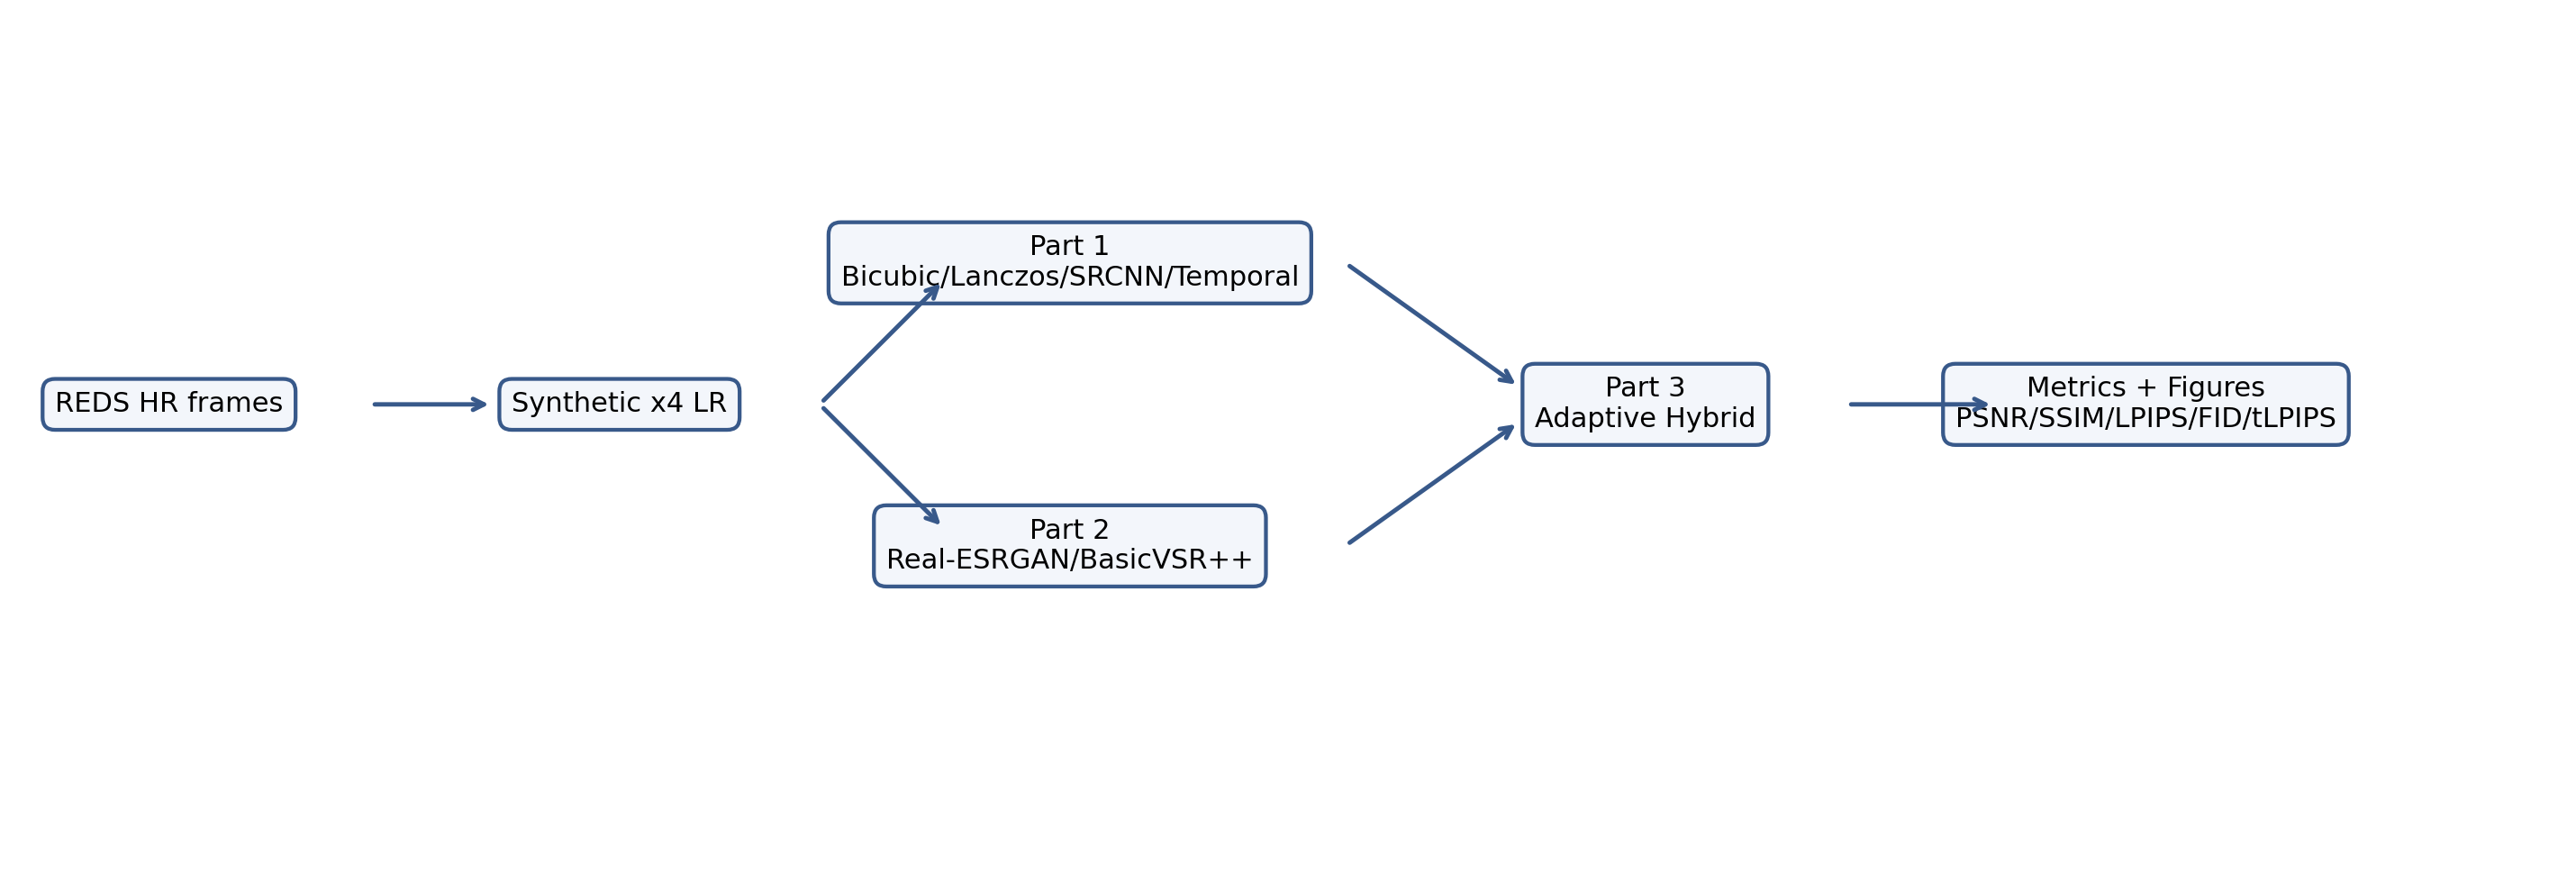
\includegraphics[width=0.85\textwidth]{pipeline_flowchart.png}
  \caption{Overall experimental pipeline. HR frames are synthetically degraded to x4 LR inputs, processed by Part~1 baselines, Part~2 pretrained methods, and Part~3 adaptive fusion, then evaluated with pixel, perceptual, temporal, and qualitative metrics.}
  \label{fig:pipeline}
\end{figure*}

\section{Experiments}
\label{sec:experiments}
\subsection{Datasets}
\textbf{Mandatory sample data.}
We use the provided REDS-sample clip \texttt{REDS\_002} with 100 frames and the Vimeo clip \texttt{00018/0043} with 7 frames. For both datasets, HR frames are downsampled by x4 to create synthetic LR inputs, so GT is available for PSNR and SSIM.

\textbf{Wild video.}
We also process a real LR wild video extracted into frame images. Since no GT is available, this dataset is used for qualitative comparison and processed video submission only.

\textbf{Full REDS validation benchmark.}
For stronger evaluation, we run the full REDS validation split, \texttt{REDS\_000} through \texttt{REDS\_029}, with 30 sequences and 100 frames per sequence. Each sequence is evaluated with seven methods: Bicubic, Lanczos, SRCNN, Temporal Average, Real-ESRGAN, BasicVSR++, and Adaptive Hybrid. This produces 210 processed videos.

\subsection{Metrics}
We report PSNR and SSIM for pixel fidelity. PSNR measures mean squared error in pixel space, while SSIM measures structural similarity and is more sensitive to local contrast and luminance consistency. LPIPS measures perceptual similarity using deep features, where lower values indicate closer perceptual match. FID is computed between restored and GT frame distributions as a supplementary perceptual indicator. For temporal consistency, we compute a warpless tLPIPS proxy: the absolute difference between consecutive-frame LPIPS changes in restored frames and GT frames. Lower LPIPS, FID, and tLPIPS are better. We use this lightweight proxy because computing optical-flow-aligned temporal perceptual distance over the full REDS validation split would substantially increase runtime.

\subsection{Implementation Details}
All experiments are implemented in Python with PyTorch, OpenCV, PIL, BasicSR, Real-ESRGAN, LPIPS, and pytorch-fid. SRCNN is run on bicubic-upsampled frames. BasicVSR and BasicVSR++ process complete sequences to preserve temporal propagation. Real-ESRGAN processes frames independently with tiled inference. For full REDS validation, metrics are computed on 30 frames per sequence for LPIPS/tLPIPS and up to 50 frames per sequence for FID to keep the benchmark feasible. All methods still generate processed videos for every frame.

\subsection{Part 1 and Part 2 Sample Results}
Table~\ref{tab:sample} summarizes the mandatory sample quantitative results. On REDS\_002, Lanczos slightly improves over Bicubic among classical baselines. SRCNN underperforms interpolation in this run, likely because the provided weights are limited. Temporal averaging performs poorly on REDS because neighboring frames are not aligned before averaging. BasicVSR and BasicVSR++ substantially improve PSNR/SSIM, confirming the value of temporal propagation and alignment. Real-ESRGAN has lower PSNR/SSIM because perceptual textures do not necessarily match GT pixels.

Fig.~\ref{fig:part1} shows the Part~1 behavior directly. The LR input contains little recoverable high-frequency information; Bicubic and Lanczos produce smooth but stable HR frames. SRCNN does not introduce strong temporal artifacts, but its shallow capacity and limited weights make its output less competitive than interpolation. Temporal averaging is visually smooth but can wash out moving structures because no optical flow or deformable alignment is used. This failure case is important: it explains why later video SR methods explicitly align or propagate features over time.

\begin{table*}[t]
\centering
\small
\caption{Sample-dataset PSNR/SSIM results. Higher is better.}
\label{tab:sample}
\begin{tabular}{llccc}
\toprule
Dataset & Method & Frames & PSNR & SSIM \\
\midrule
\multirow{7}{*}{REDS\_002}
& Bicubic & 100 & 21.6300 & 0.675386 \\
& Lanczos & 100 & 21.8382 & 0.687649 \\
& SRCNN & 100 & 20.5023 & 0.652510 \\
& Temporal Avg. & 100 & 20.3740 & 0.595532 \\
& Real-ESRGAN & 100 & 19.8416 & 0.632718 \\
& BasicVSR & 100 & 26.1518 & 0.883018 \\
& BasicVSR++ & 100 & 26.8504 & 0.900157 \\
\midrule
\multirow{7}{*}{Vimeo}
& Bicubic & 7 & 27.5722 & 0.751740 \\
& Lanczos & 7 & 27.7183 & 0.759160 \\
& SRCNN & 7 & 24.2808 & 0.690225 \\
& Temporal Avg. & 7 & 27.6853 & 0.758837 \\
& Real-ESRGAN & 7 & 24.9929 & 0.667951 \\
& BasicVSR & 7 & 29.1144 & 0.830463 \\
& BasicVSR++ & 7 & 29.3056 & 0.834918 \\
\bottomrule
\end{tabular}
\end{table*}

\begin{figure}[t]
  \centering
  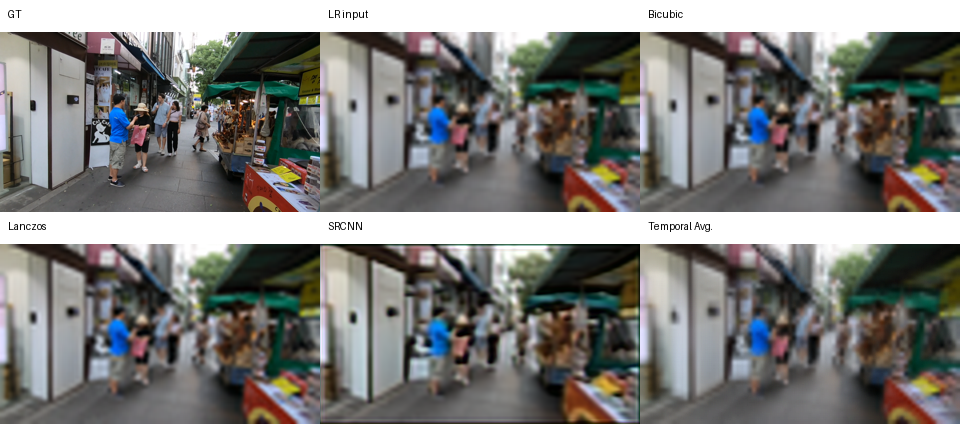
\includegraphics[width=\linewidth]{part1_reds002_grid.png}
  \caption{Part~1 baseline comparison on REDS\_002. Classical interpolation is stable but blurry; naive temporal averaging can suppress detail when frames are not aligned.}
  \label{fig:part1}
\end{figure}

\begin{figure}[t]
  \centering
  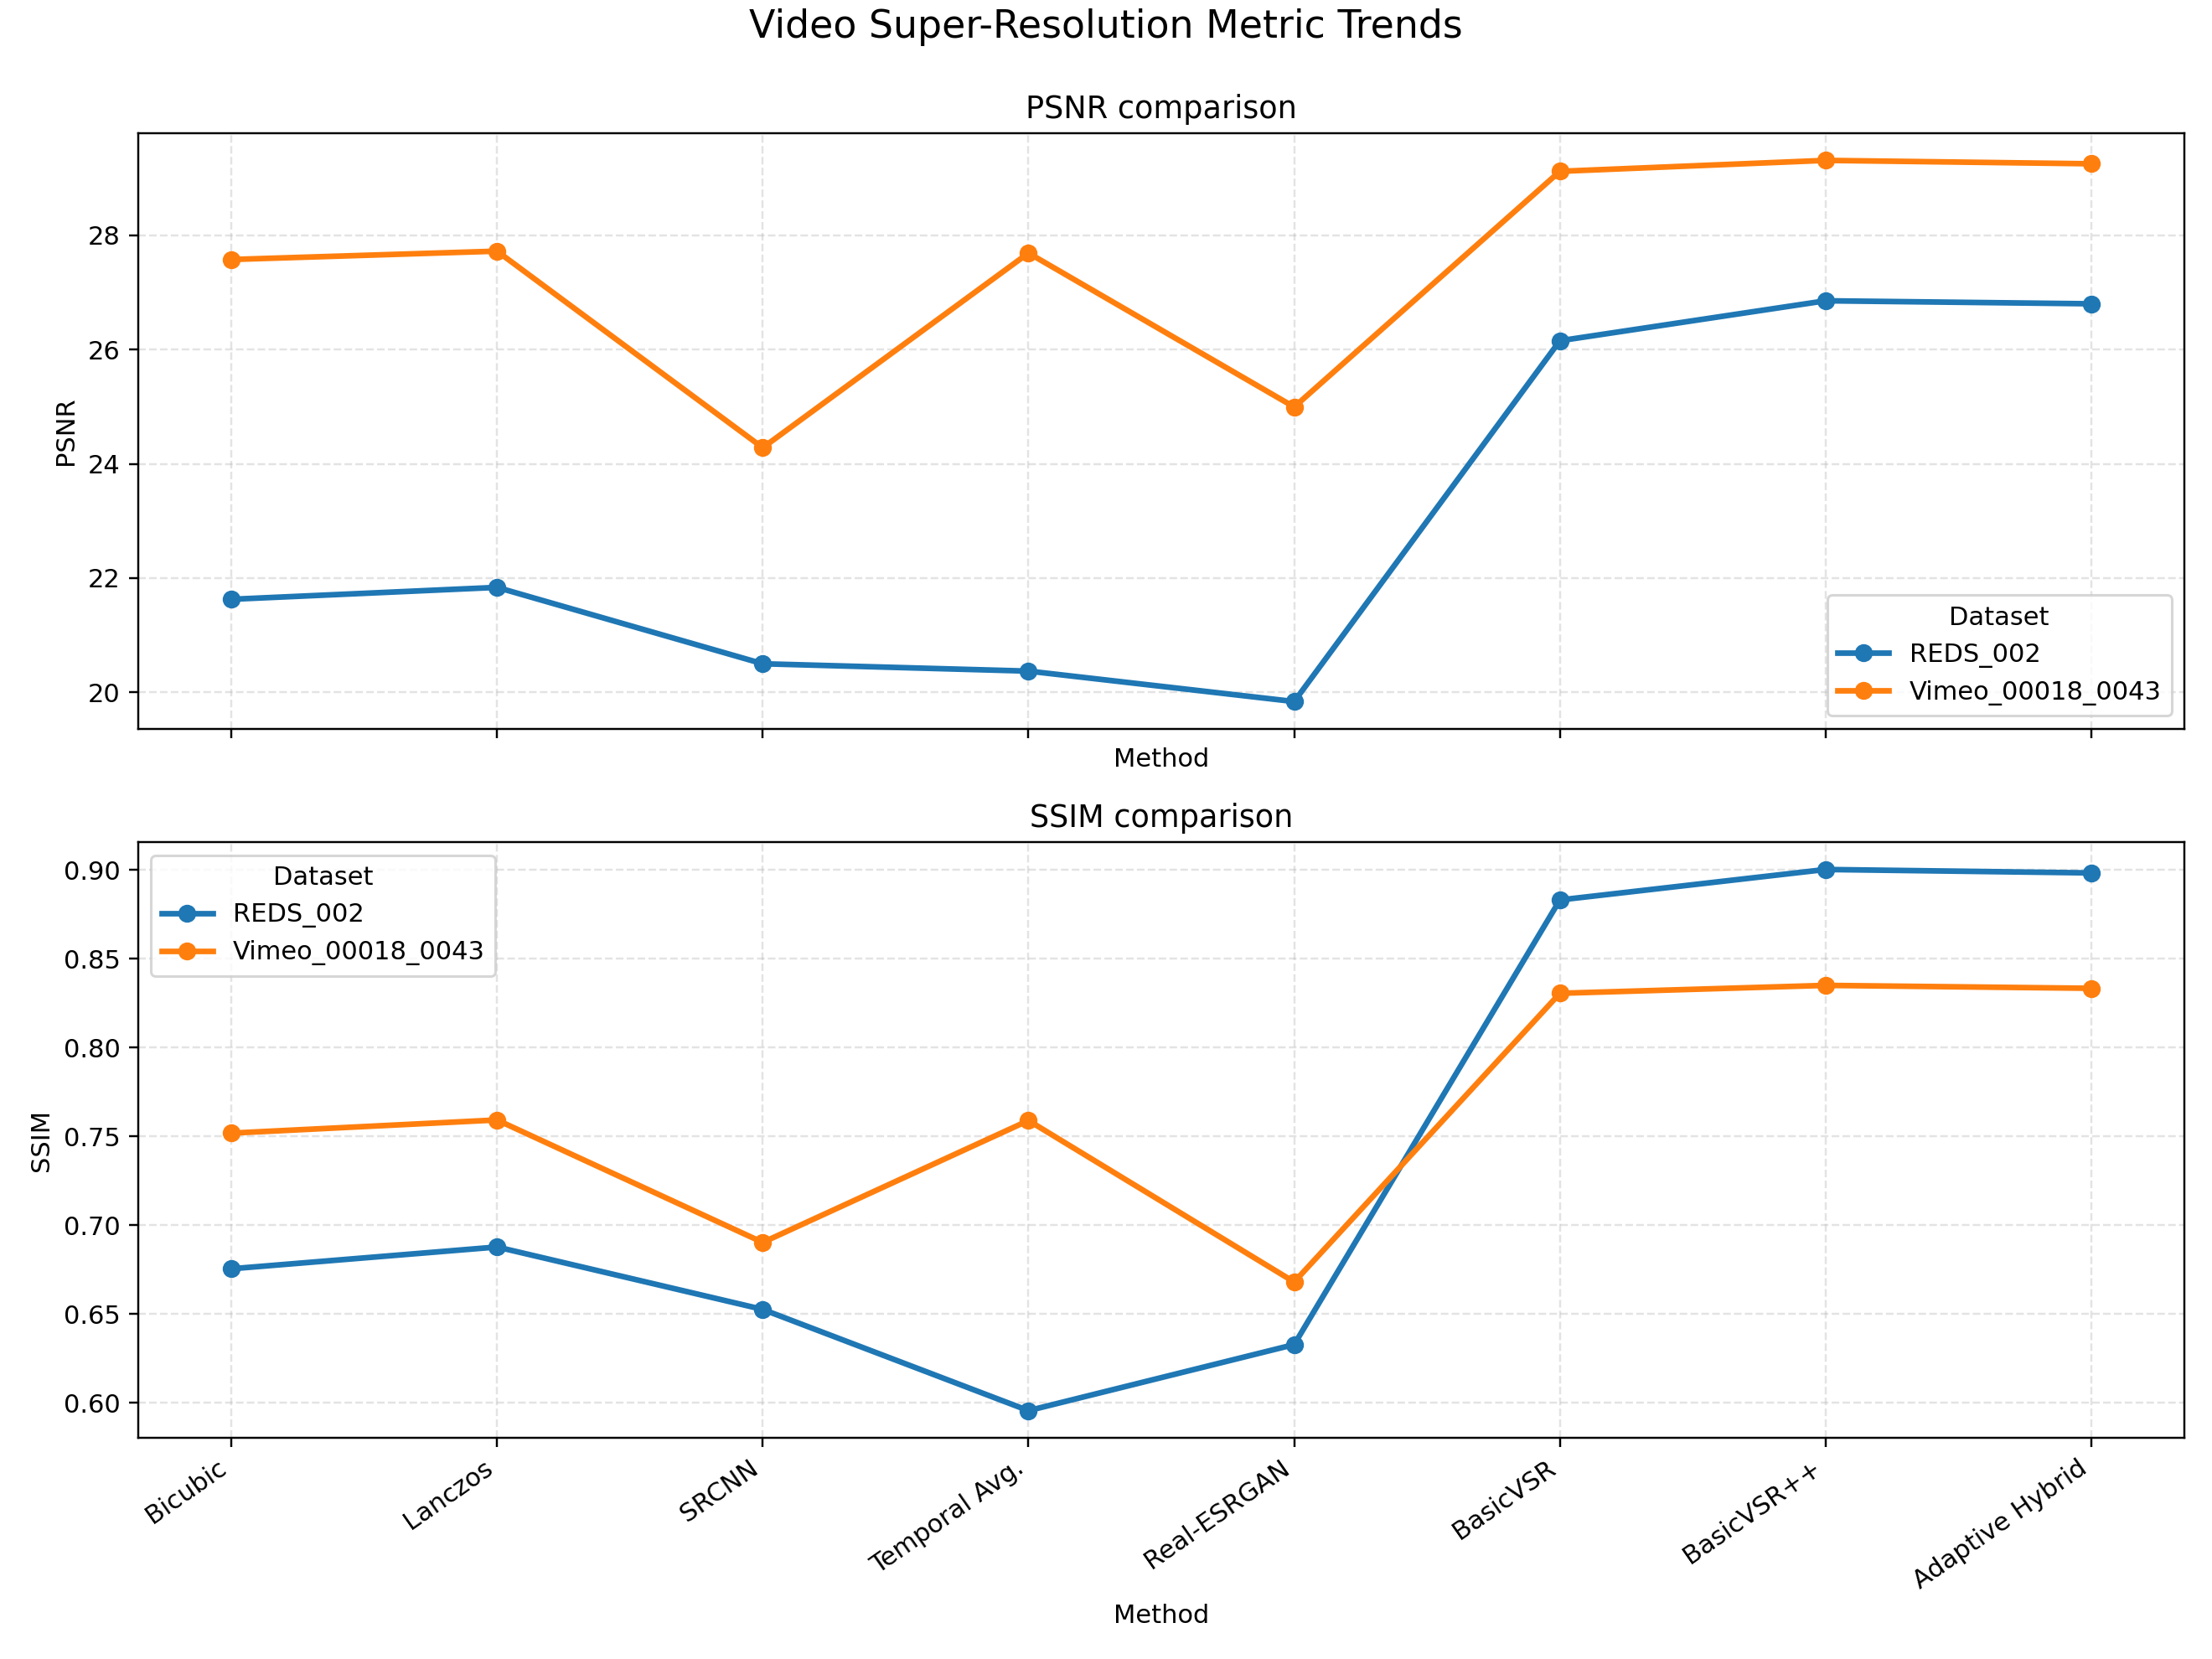
\includegraphics[width=\linewidth]{sample_metric_line.png}
  \caption{Mandatory sample PSNR/SSIM trends over Part~1, Part~2, and Part~3 methods. BasicVSR and BasicVSR++ improve distortion metrics by exploiting temporal propagation.}
  \label{fig:sampletrends}
\end{figure}

\subsection{Part 3 Sample Results}
The adaptive hybrid is not designed to maximize PSNR/SSIM beyond BasicVSR++. Instead, it preserves most of the BasicVSR++ structure while incorporating a controlled amount of Real-ESRGAN detail. On REDS\_002, the hybrid reaches 26.7978 PSNR and 0.898219 SSIM, close to BasicVSR++ at 26.8504 and 0.900157. On Vimeo, the hybrid reaches 29.2463 PSNR and 0.833274 SSIM, again close to BasicVSR++.

Fig.~\ref{fig:samplemethods} compares representative outputs from the mandatory REDS sample. Real-ESRGAN produces stronger texture and contrast, but the generated details do not always match the GT frame. BasicVSR and BasicVSR++ better preserve the global structure, with BasicVSR++ producing the best distortion-oriented reconstruction. The hybrid result is visually close to BasicVSR++ because the mask keeps the stable backbone dominant.

\begin{figure}[t]
  \centering
  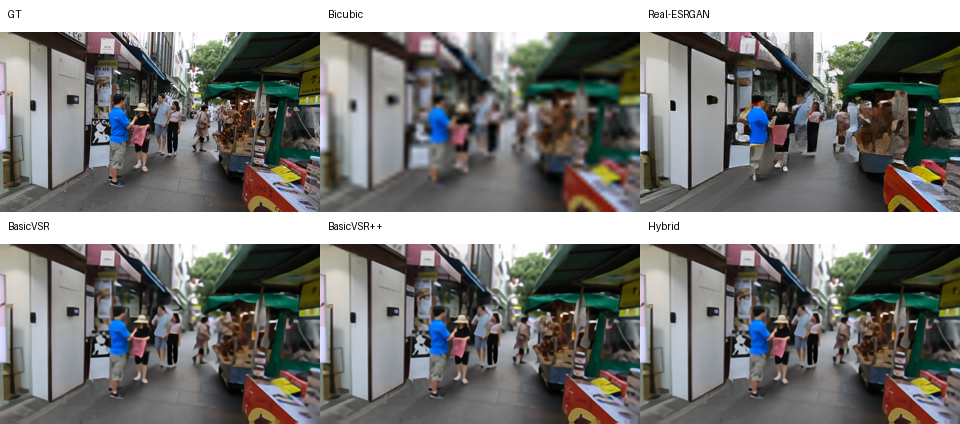
\includegraphics[width=\linewidth]{sample_methods_reds002_grid.png}
  \caption{Representative sample outputs on REDS\_002. Real-ESRGAN emphasizes perceptual texture, while BasicVSR/BasicVSR++ preserve GT-aligned structure.}
  \label{fig:samplemethods}
\end{figure}

\begin{figure}[t]
  \centering
  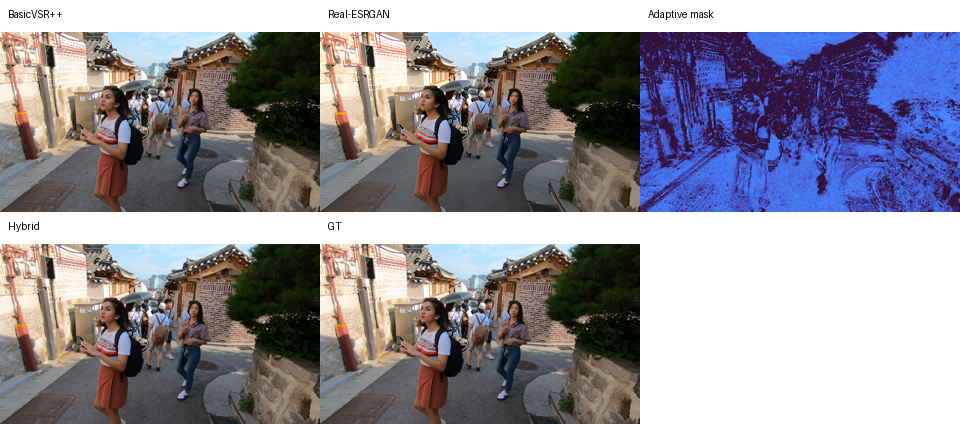
\includegraphics[width=\linewidth]{part3_fusion_grid.png}
  \caption{Part~3 adaptive hybrid example. BasicVSR++ supplies the stable reconstruction, Real-ESRGAN supplies perceptual detail, and the adaptive mask controls local fusion.}
  \label{fig:part3}
\end{figure}

\begin{figure}[t]
  \centering
  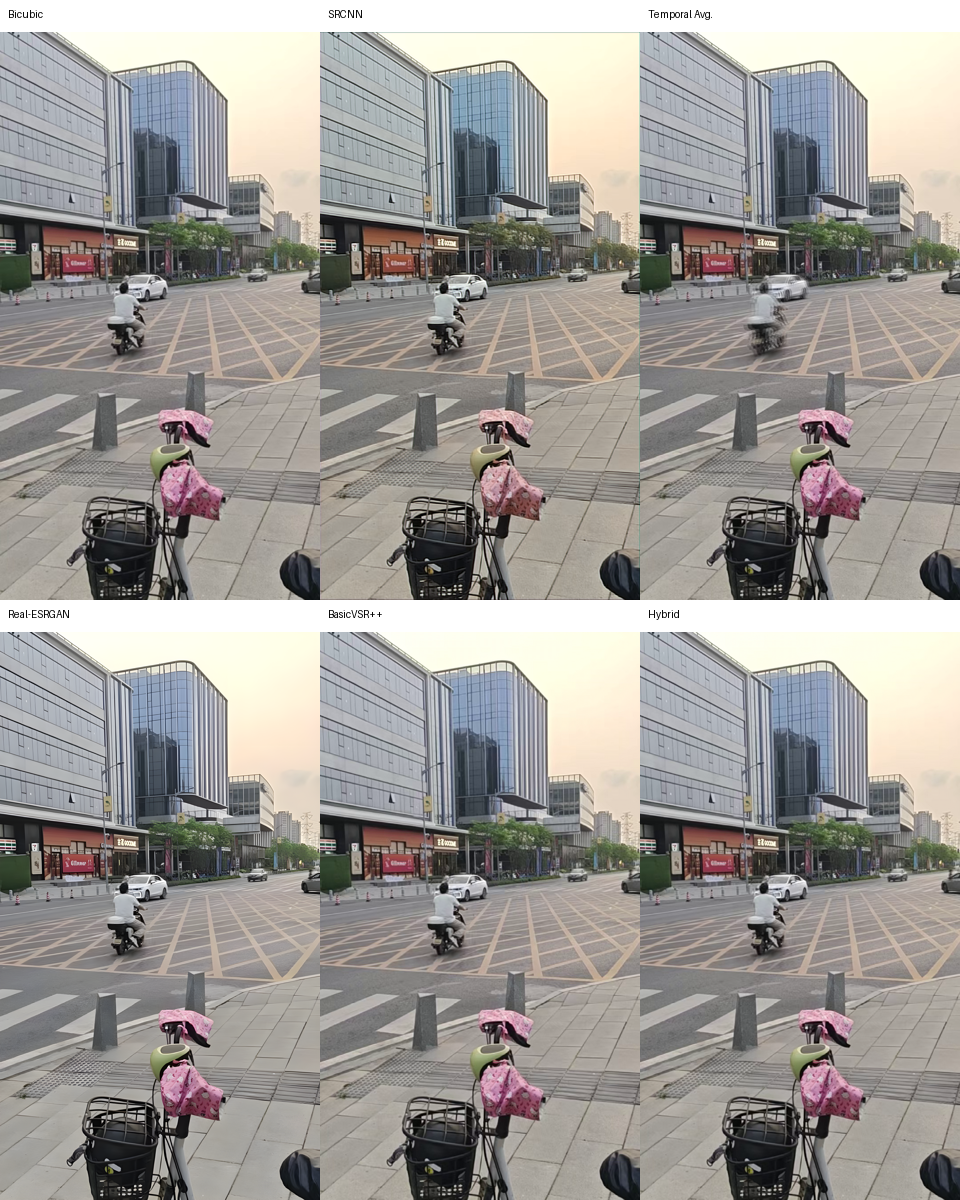
\includegraphics[width=\linewidth]{wild_methods_grid.png}
  \caption{Qualitative comparison on real wild LR input without GT. This figure is used for visual inspection only; no PSNR/SSIM is reported for wild video.}
  \label{fig:wild}
\end{figure}

\subsection{Full REDS Validation Results}
Table~\ref{tab:redsfull} reports the full REDS validation benchmark. BasicVSR++ obtains the best PSNR and SSIM, showing that temporal propagation and alignment are crucial for GT-aligned VSR. The adaptive hybrid remains close to BasicVSR++ and has slightly lower LPIPS, supporting its role as a lightweight perception-distortion trade-off. Real-ESRGAN has much lower PSNR/SSIM, but it improves LPIPS and tLPIPS compared with classical baselines, which matches its perceptual restoration objective.

\begin{table*}[t]
\centering
\small
\caption{Full REDS validation benchmark averaged over 30 sequences. Higher is better for PSNR/SSIM; lower is better for LPIPS/FID/tLPIPS.}
\label{tab:redsfull}
\begin{tabular}{lccccc}
\toprule
Method & PSNR & SSIM & LPIPS & FID & tLPIPS \\
\midrule
BasicVSR++ & 31.7750 & 0.901598 & 0.156181 & 14.1000 & 0.012558 \\
Adaptive Hybrid & 31.6592 & 0.898746 & 0.155519 & 15.5069 & 0.013661 \\
Lanczos & 26.5026 & 0.741679 & 0.485979 & 73.8822 & 0.028244 \\
Bicubic & 26.2932 & 0.733447 & 0.477673 & 74.6166 & 0.028566 \\
SRCNN & 25.0887 & 0.725723 & 0.517347 & 88.2411 & 0.024511 \\
Real-ESRGAN & 24.3263 & 0.691159 & 0.225280 & 71.6246 & 0.009300 \\
Temporal Avg. & 23.1535 & 0.637528 & 0.530395 & 131.0968 & 0.085997 \\
\bottomrule
\end{tabular}
\end{table*}

\begin{figure}[t]
  \centering
  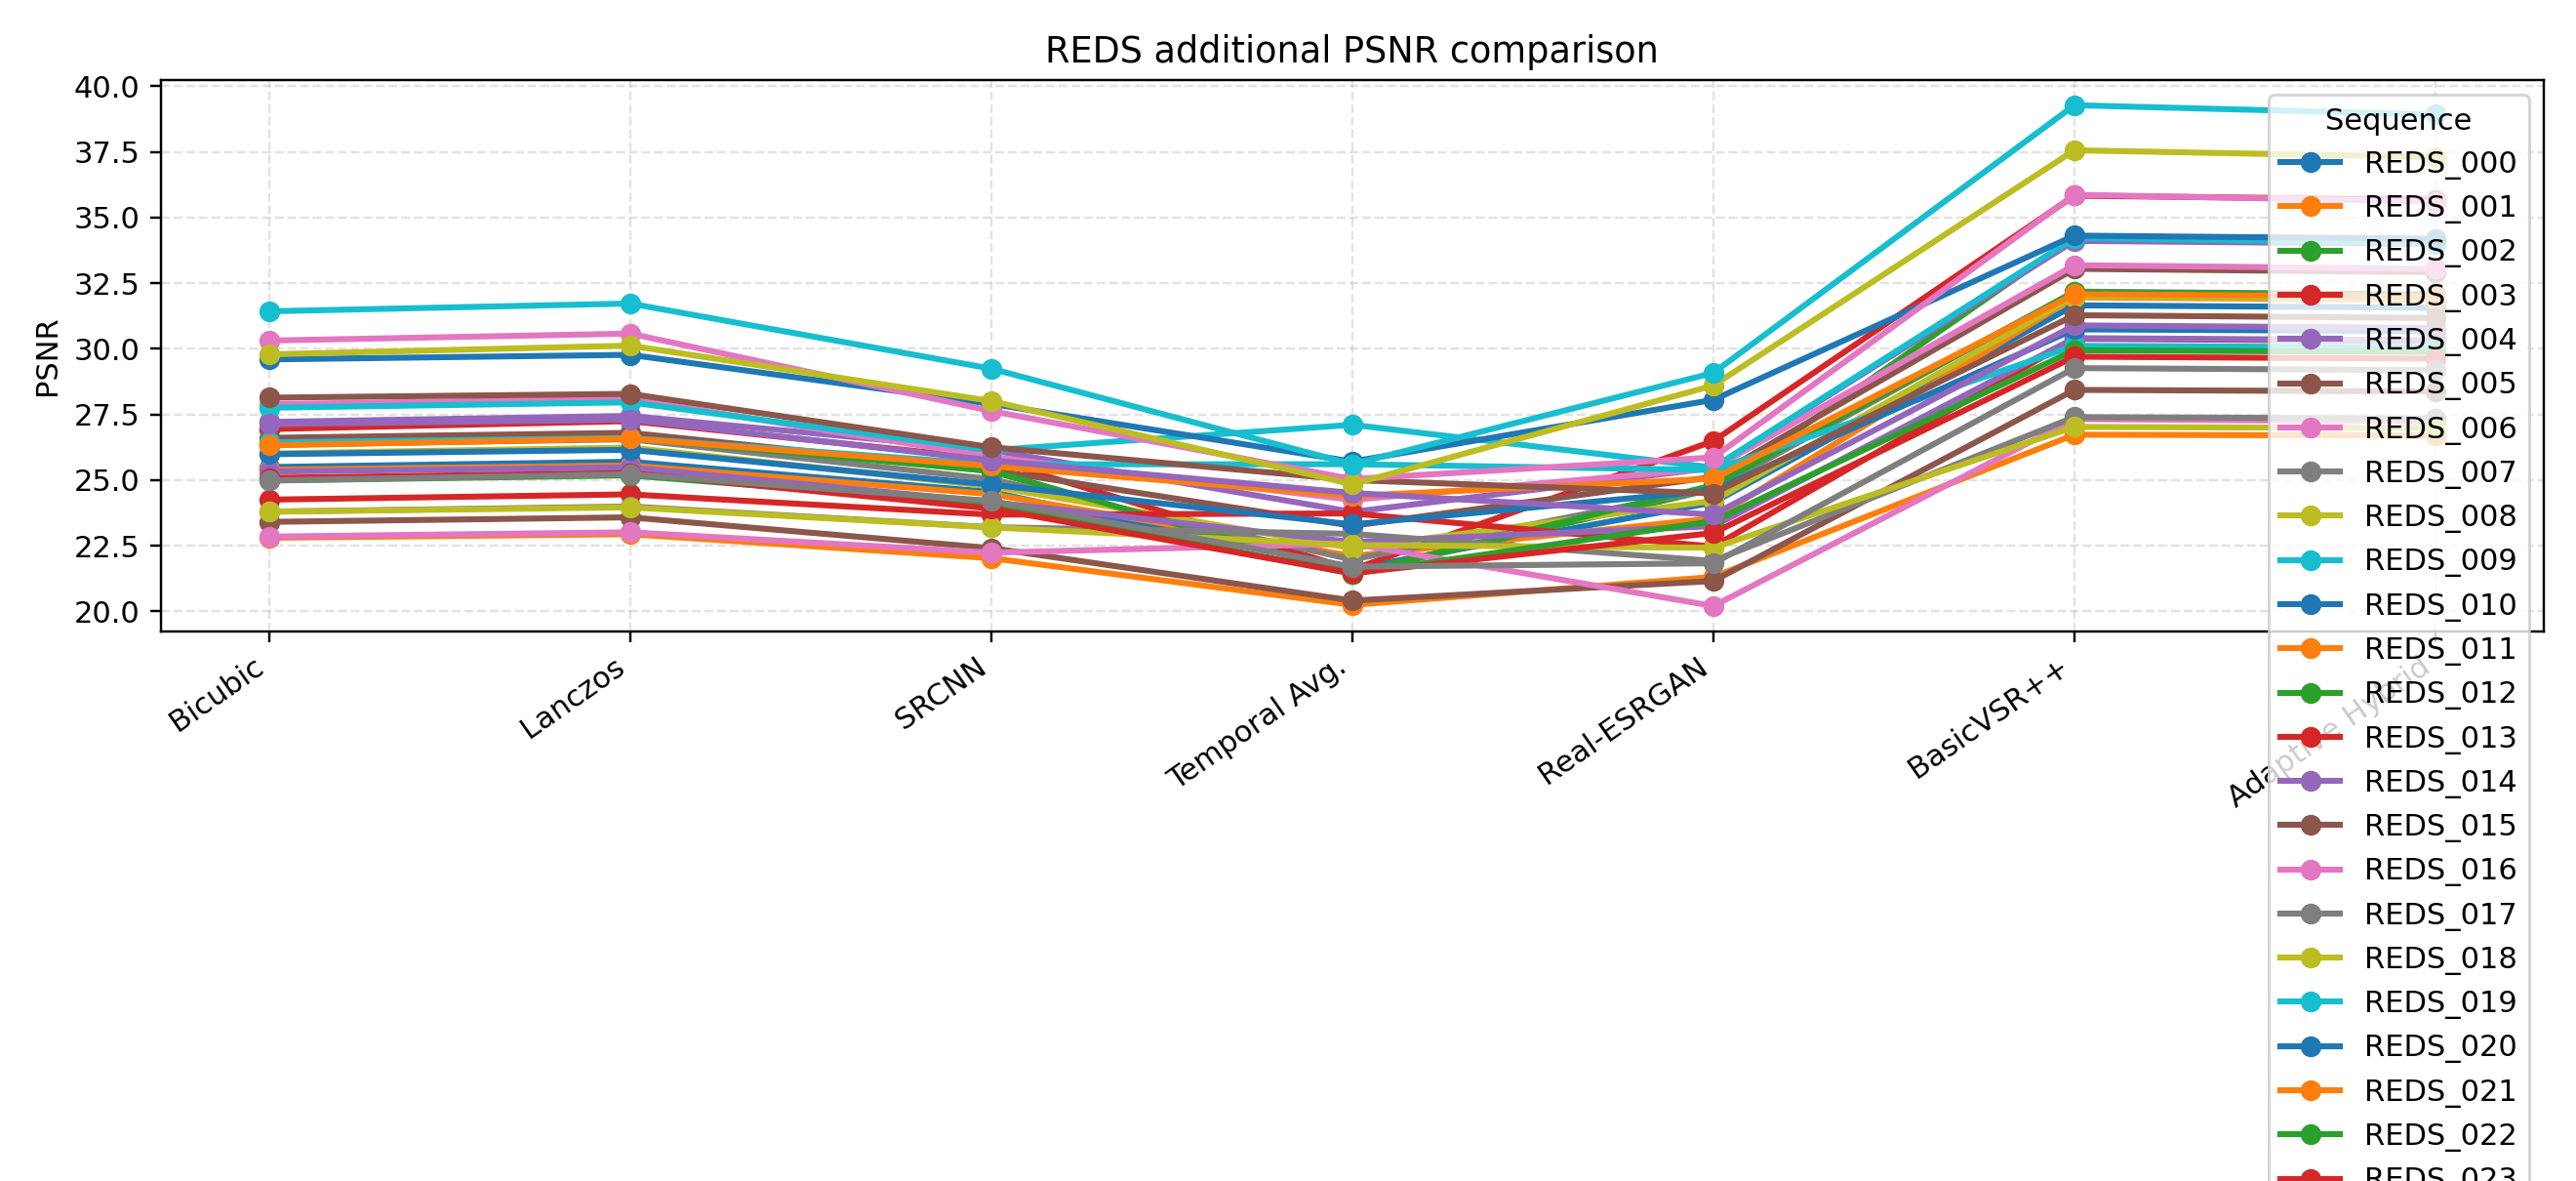
\includegraphics[width=\linewidth]{reds_psnr.png}
  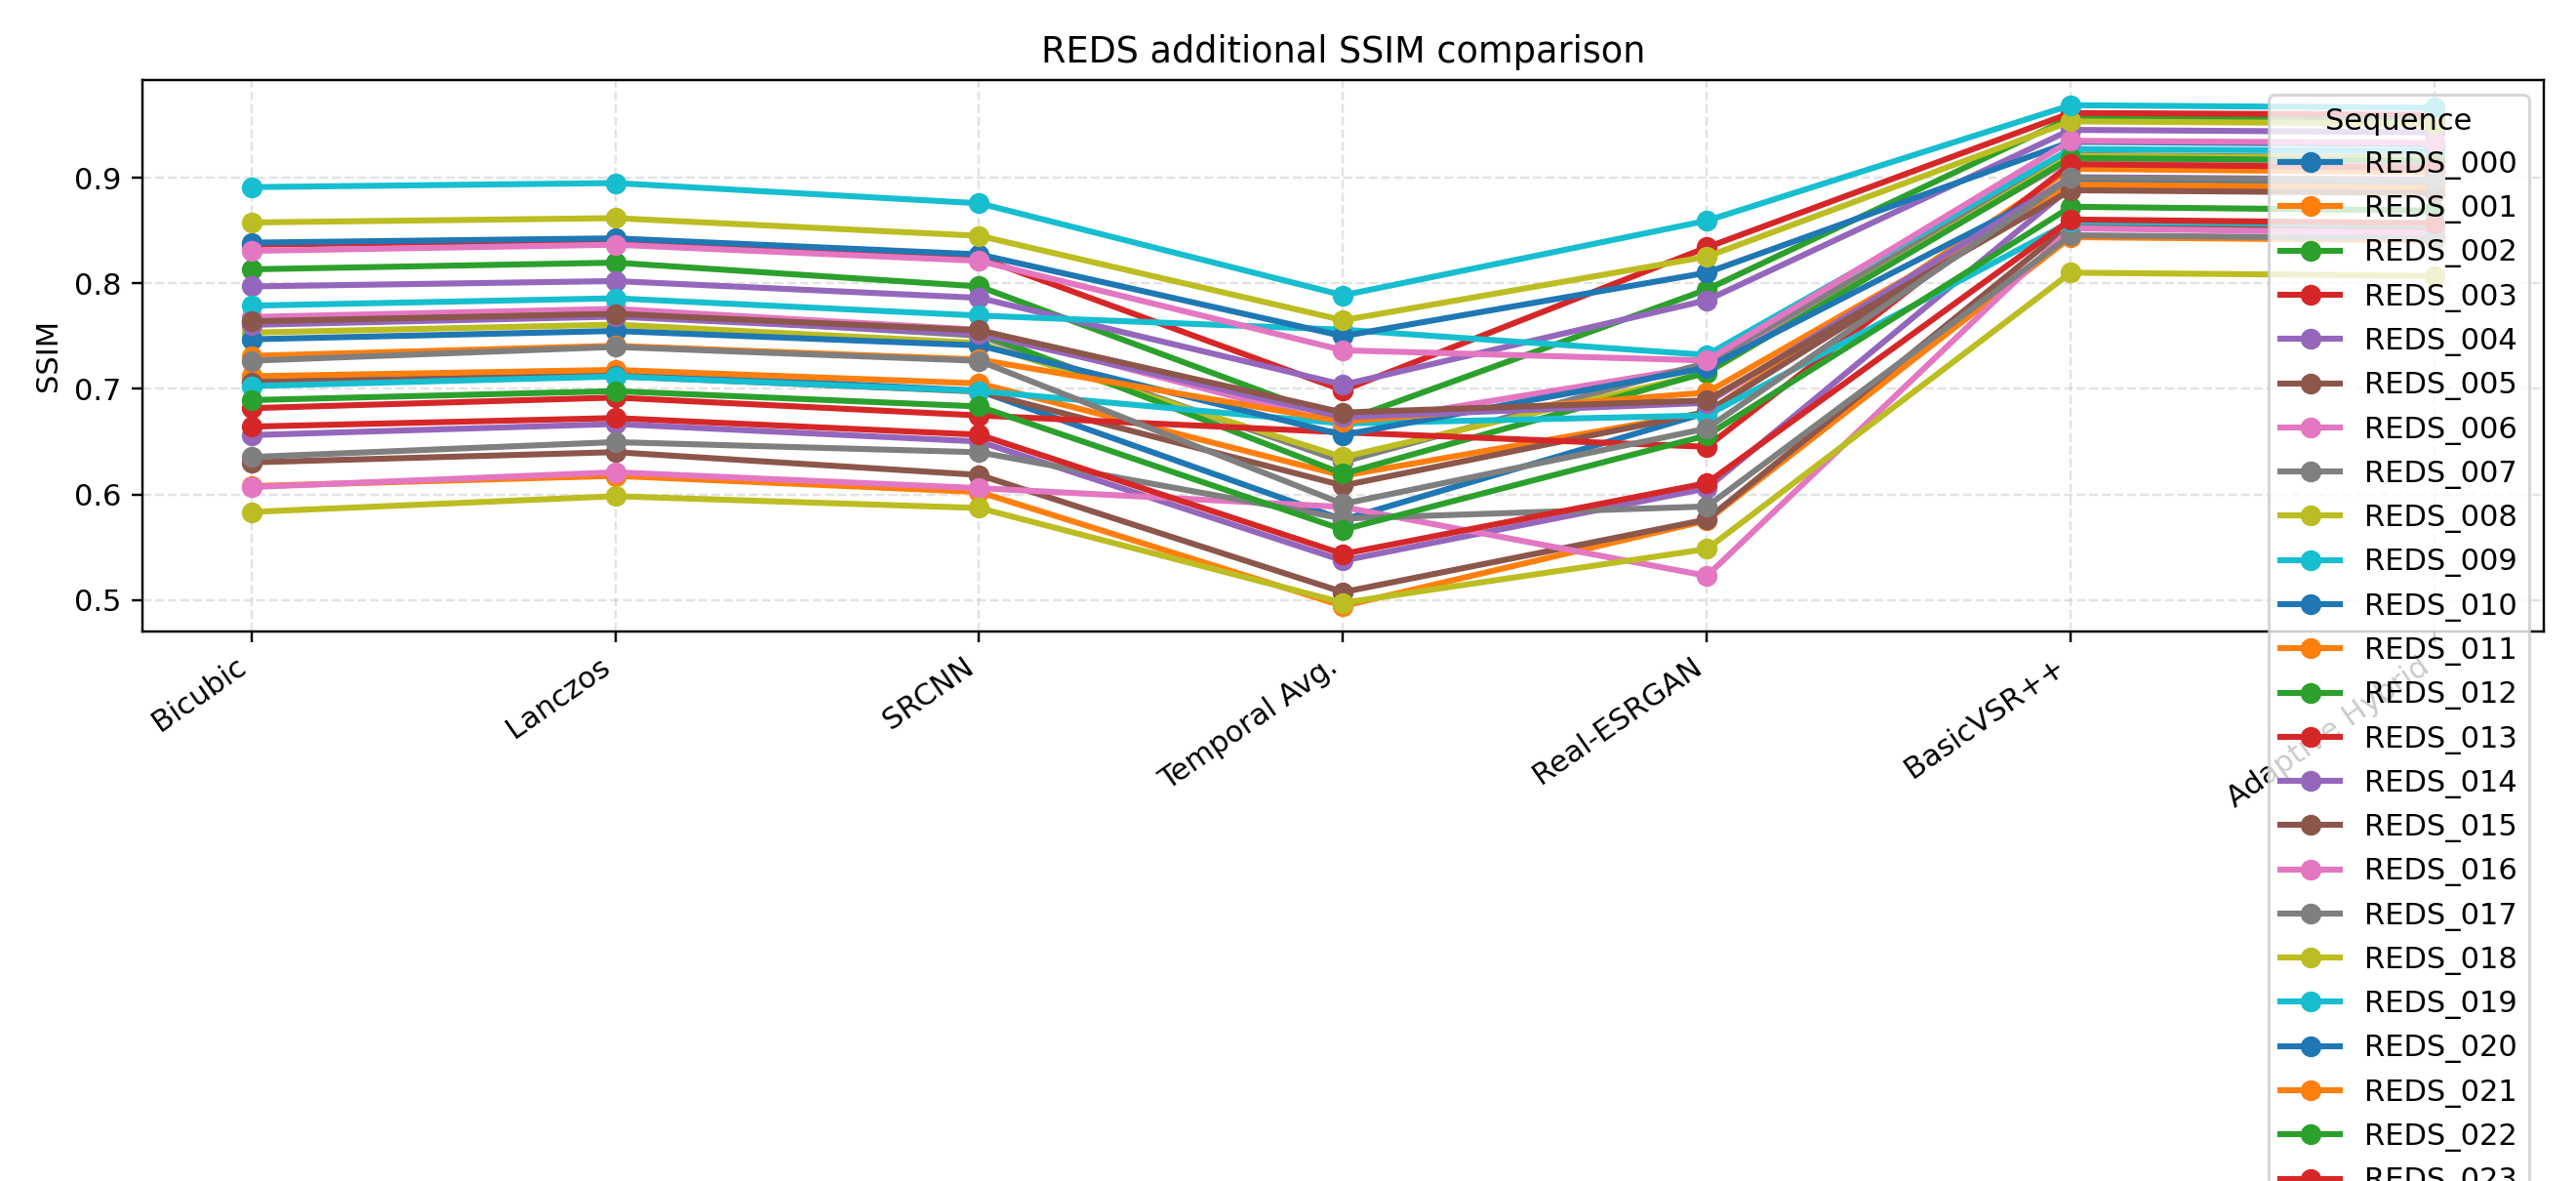
\includegraphics[width=\linewidth]{reds_ssim.png}
  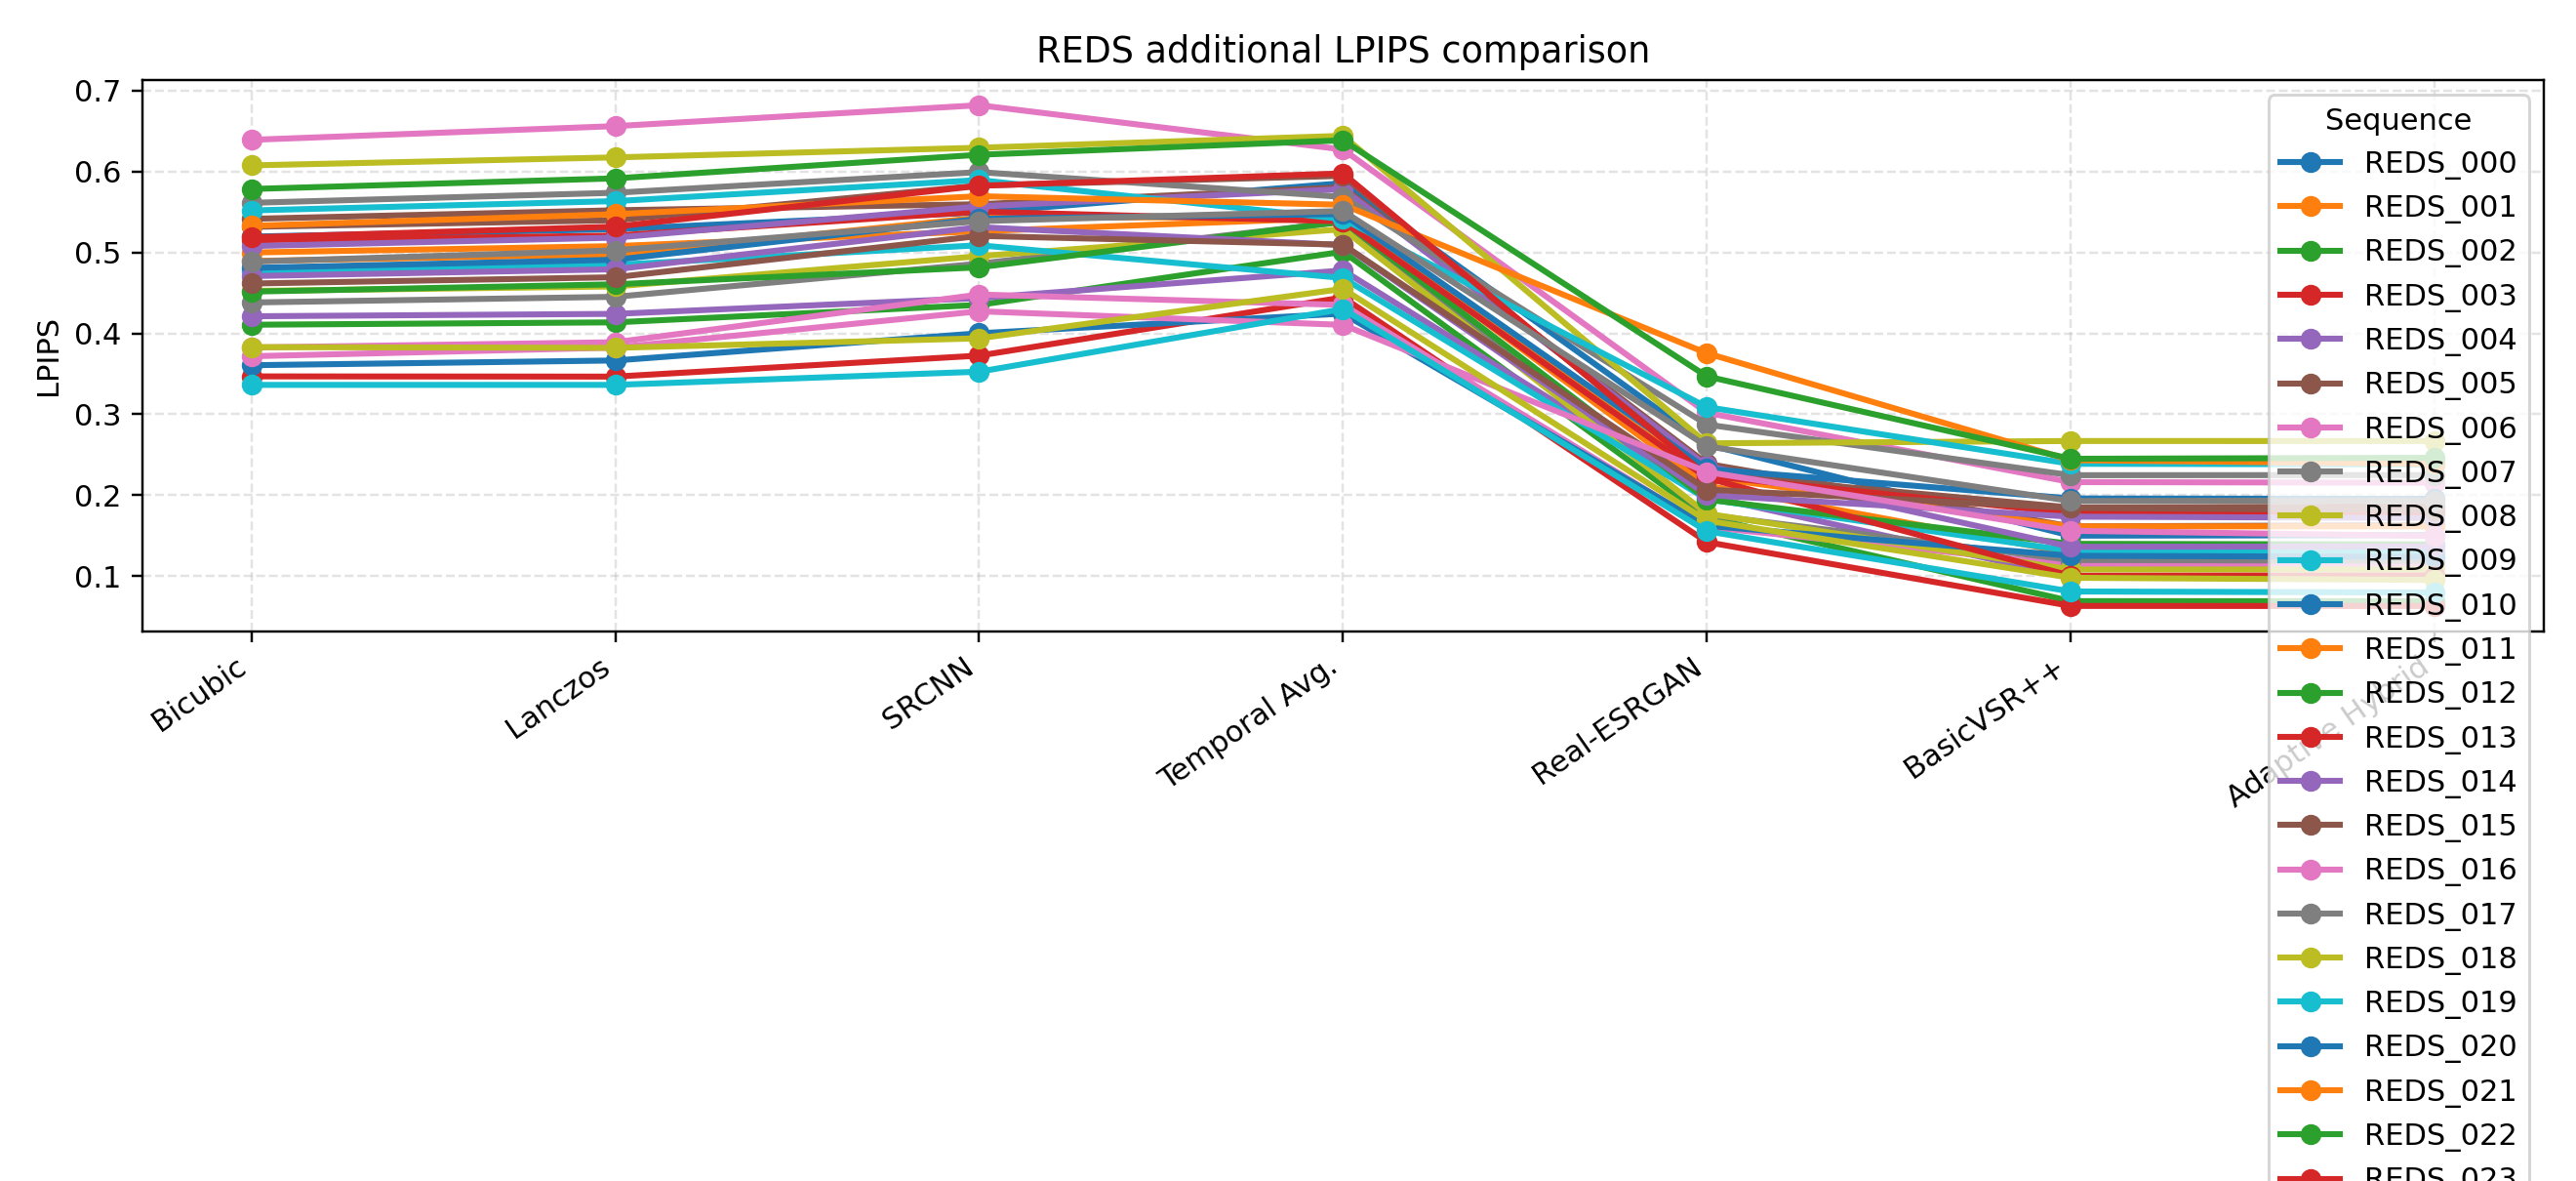
\includegraphics[width=\linewidth]{reds_lpips.png}
  \caption{Full REDS validation PSNR, SSIM, and LPIPS trends. BasicVSR++ dominates distortion metrics, while Real-ESRGAN and the adaptive hybrid show the expected perceptual-metric trade-off.}
  \label{fig:metrictrends}
\end{figure}

\begin{figure}[t]
  \centering
  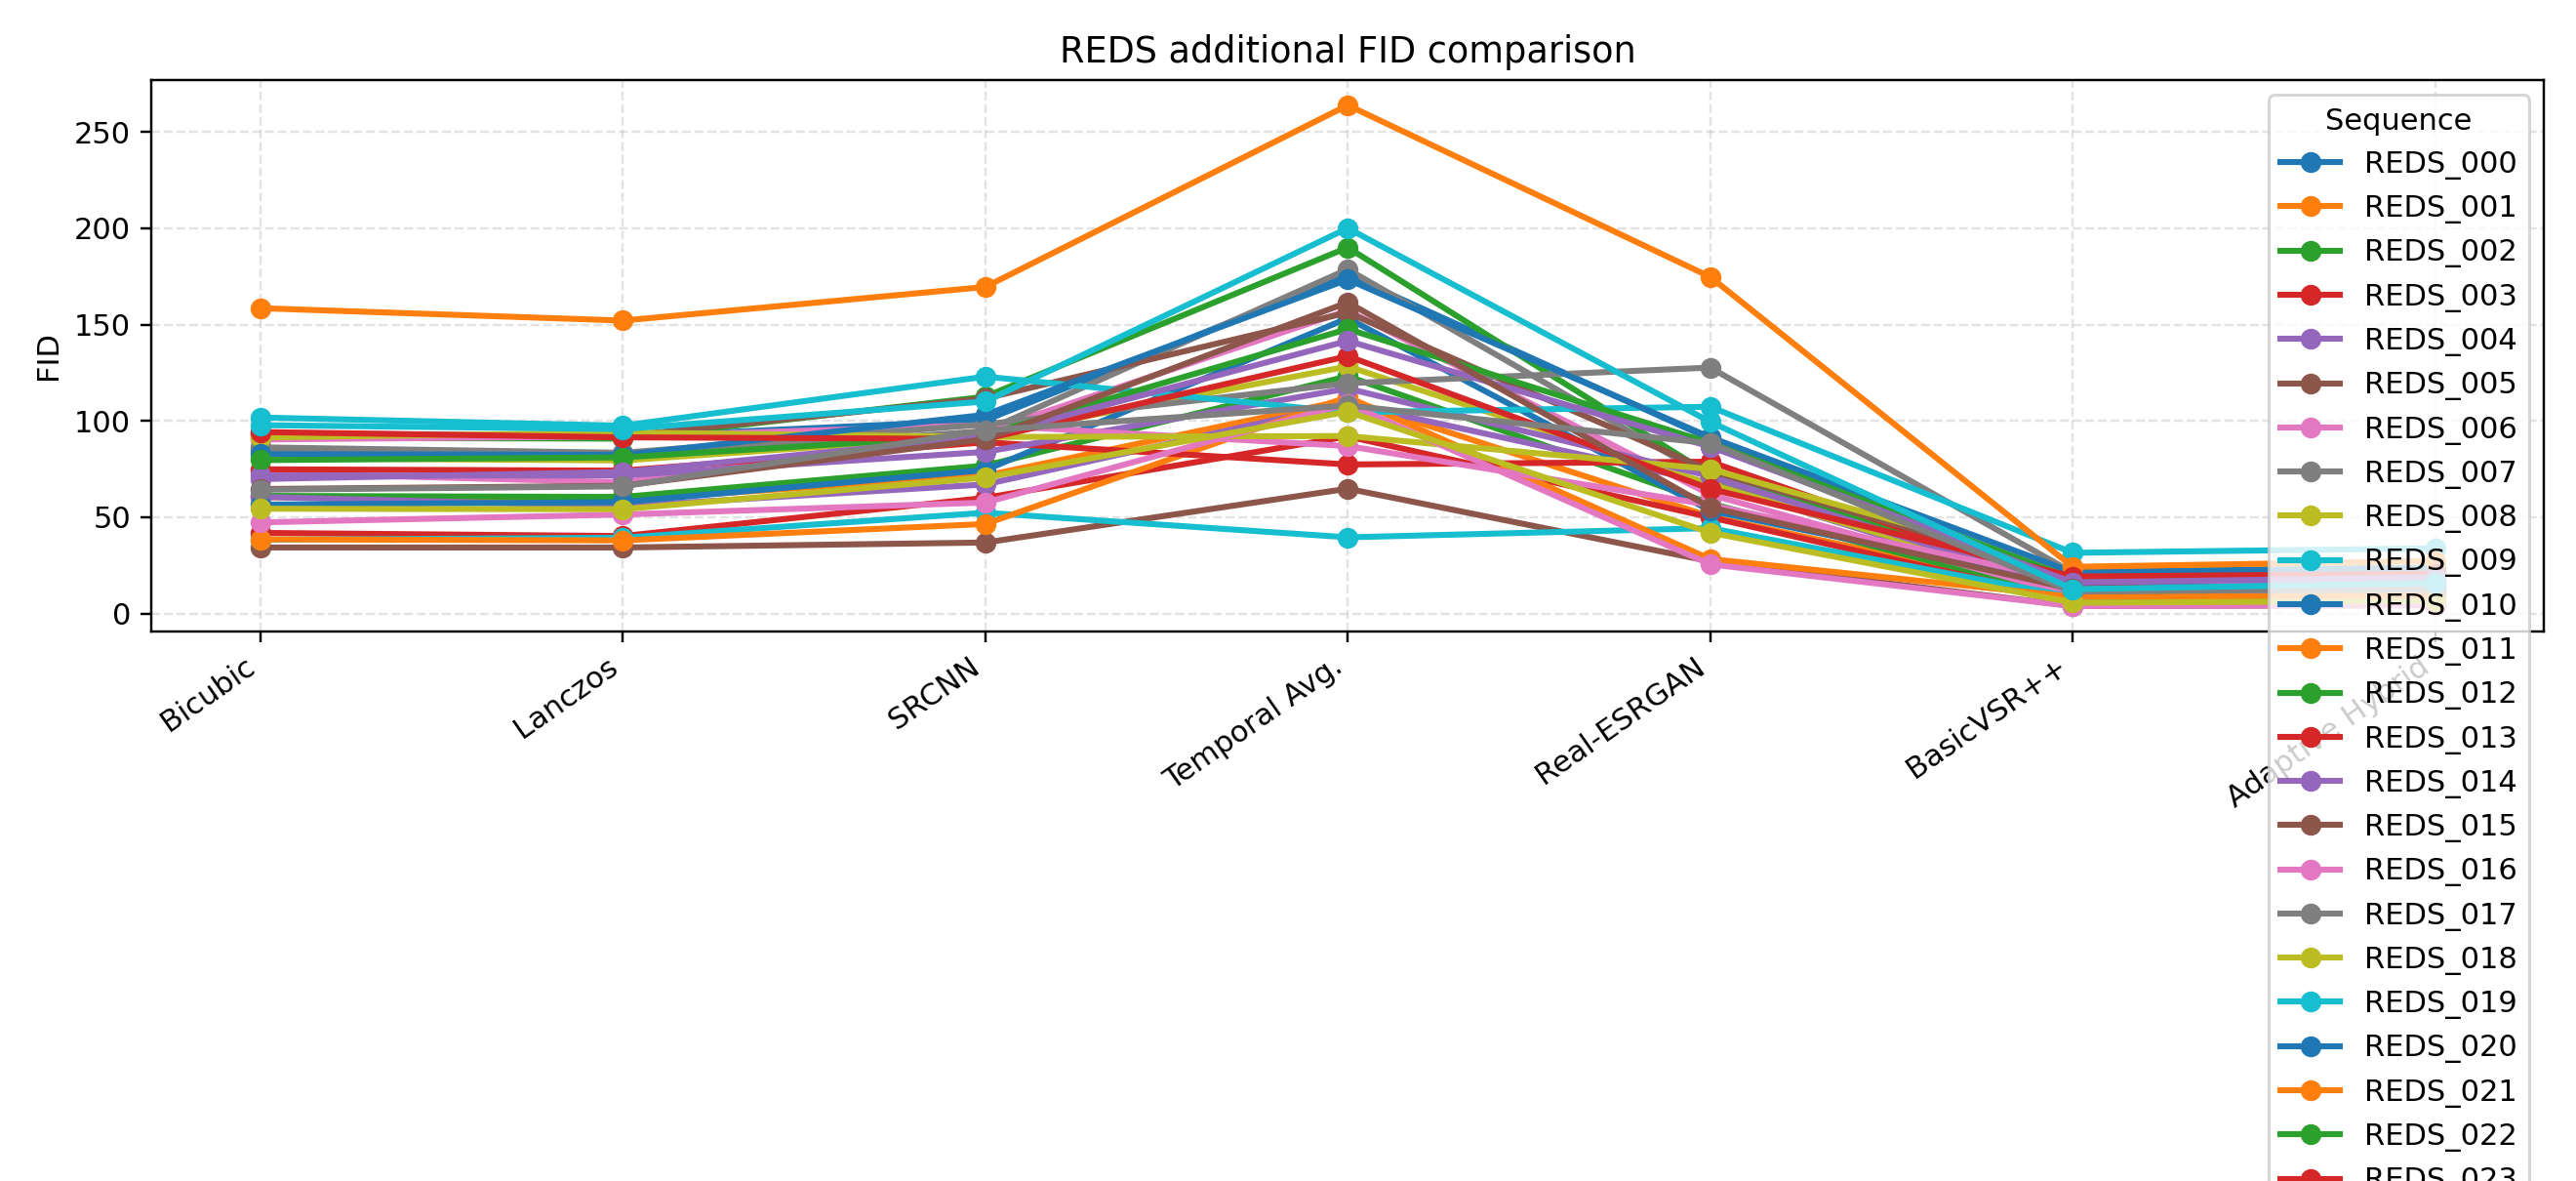
\includegraphics[width=\linewidth]{reds_fid.png}
  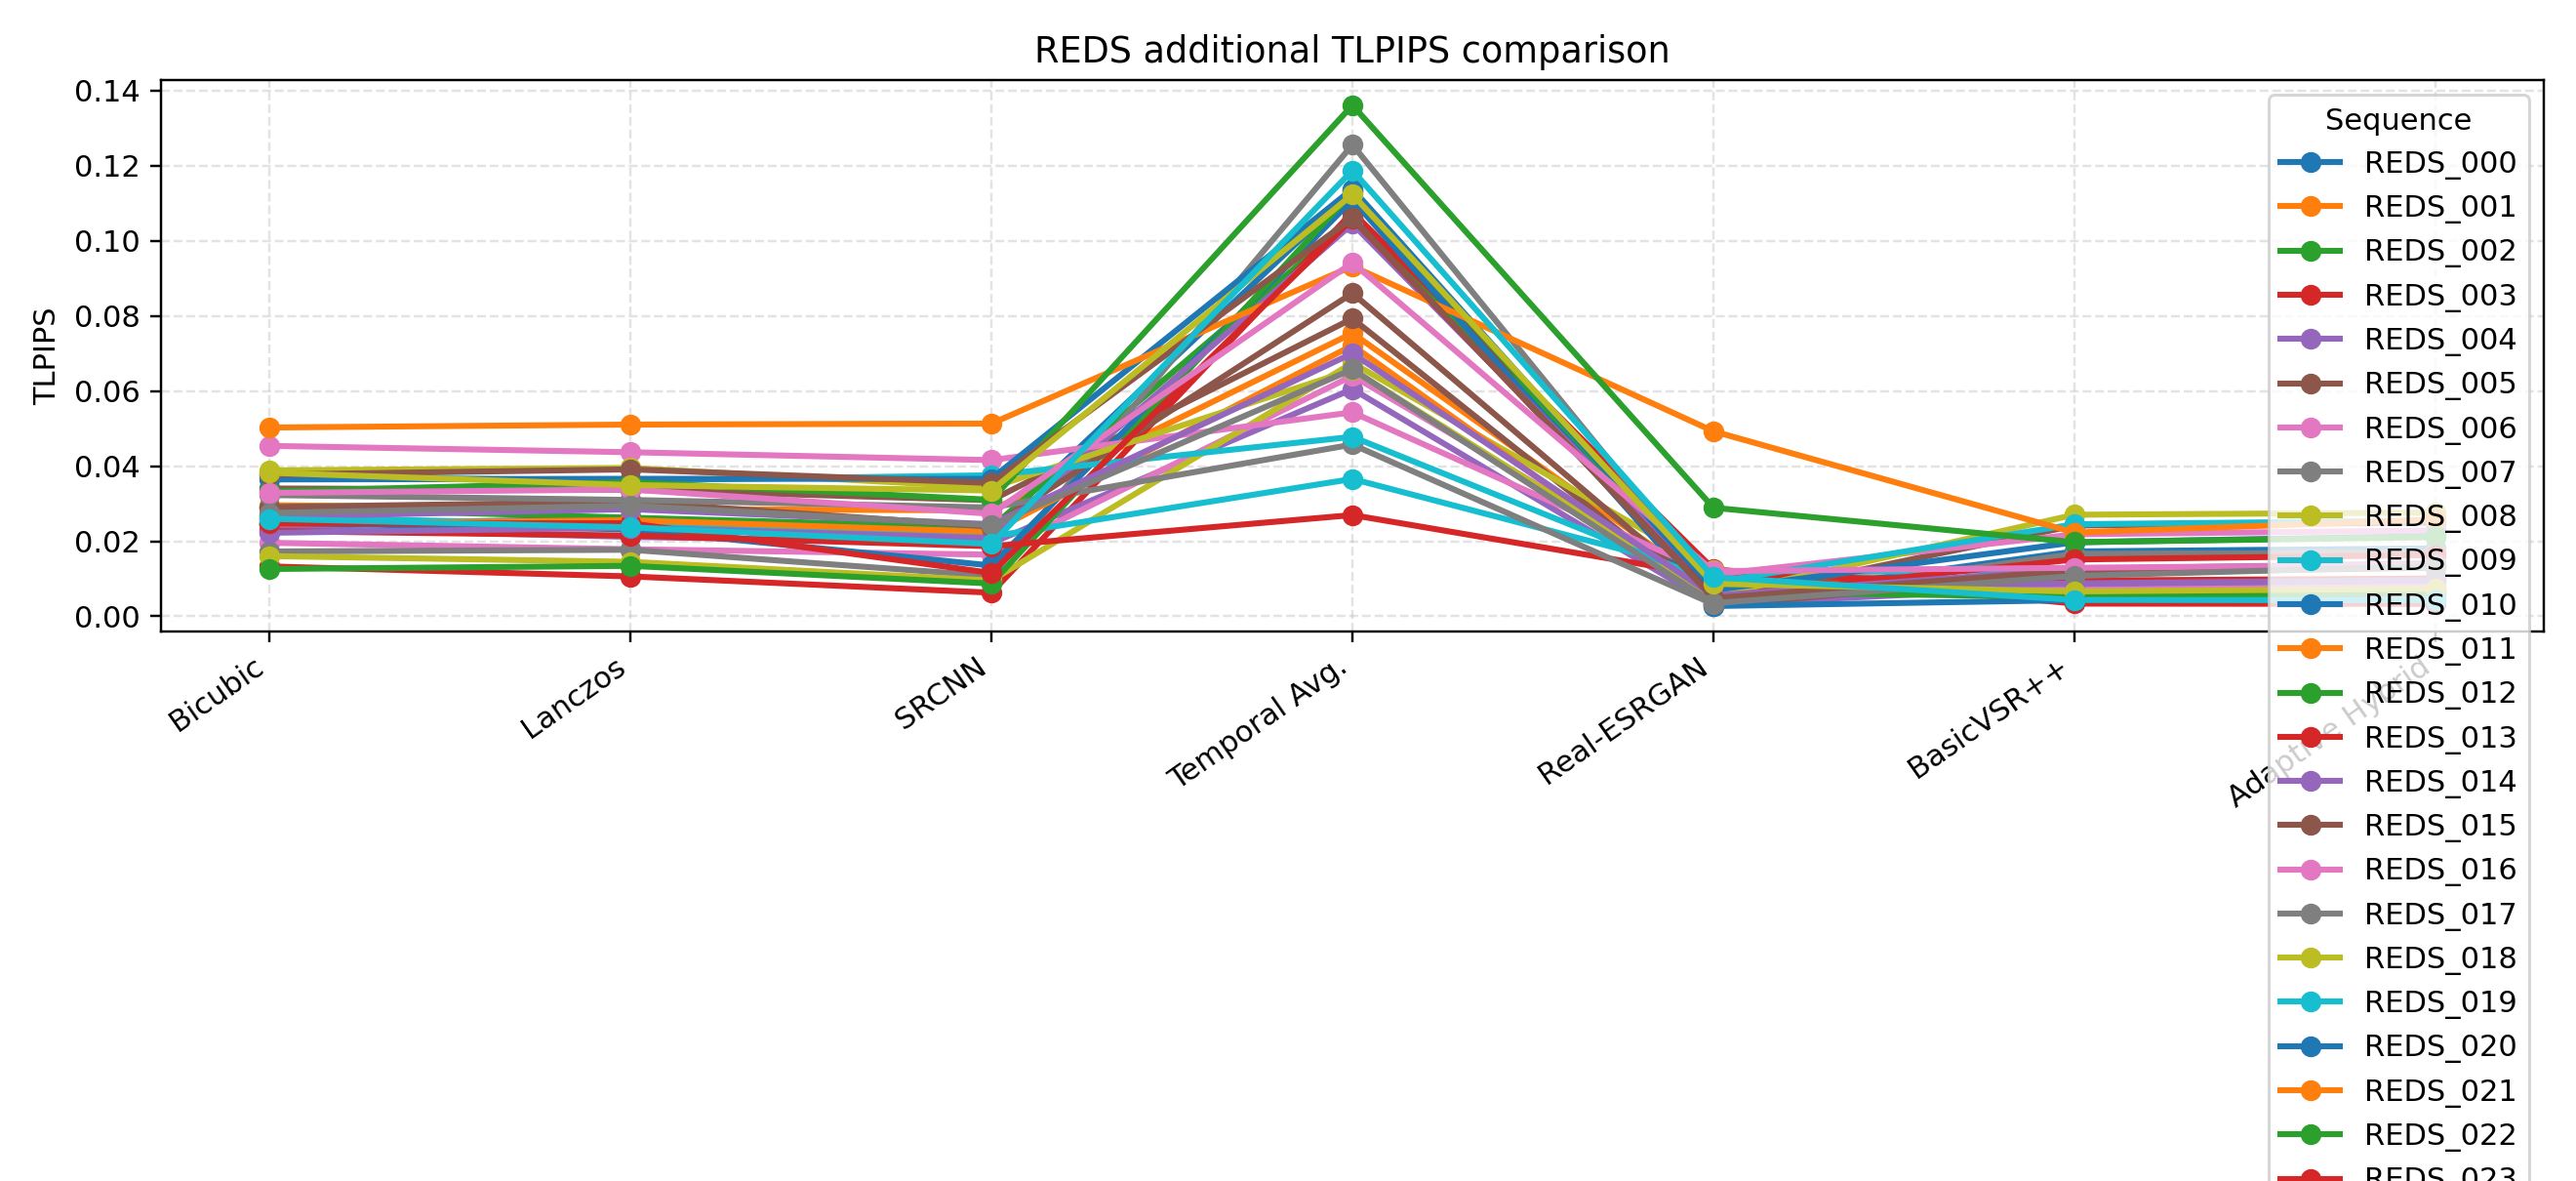
\includegraphics[width=\linewidth]{reds_tlpips.png}
  \caption{Full REDS validation perceptual-distribution and temporal-consistency trends. FID captures distribution-level perceptual differences, while tLPIPS estimates additional flicker beyond GT frame-to-frame changes.}
  \label{fig:fidtlpips}
\end{figure}

\begin{figure}[t]
  \centering
  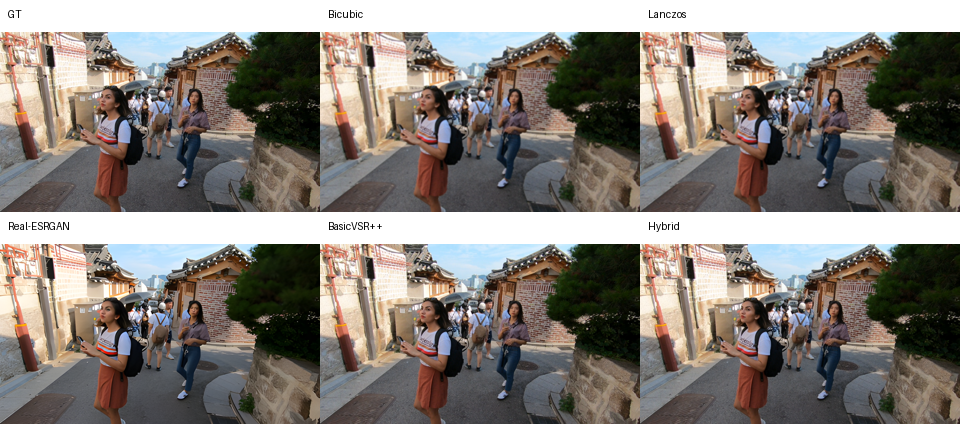
\includegraphics[width=\linewidth]{reds000_rendering_grid.png}
  \caption{Qualitative rendering comparison on REDS validation. Interpolation baselines are stable but blurry, Real-ESRGAN generates sharper perceptual texture, BasicVSR++ gives the strongest GT-aligned reconstruction, and the hybrid selectively incorporates perceptual details.}
  \label{fig:rendering}
\end{figure}

\begin{figure}[t]
  \centering
  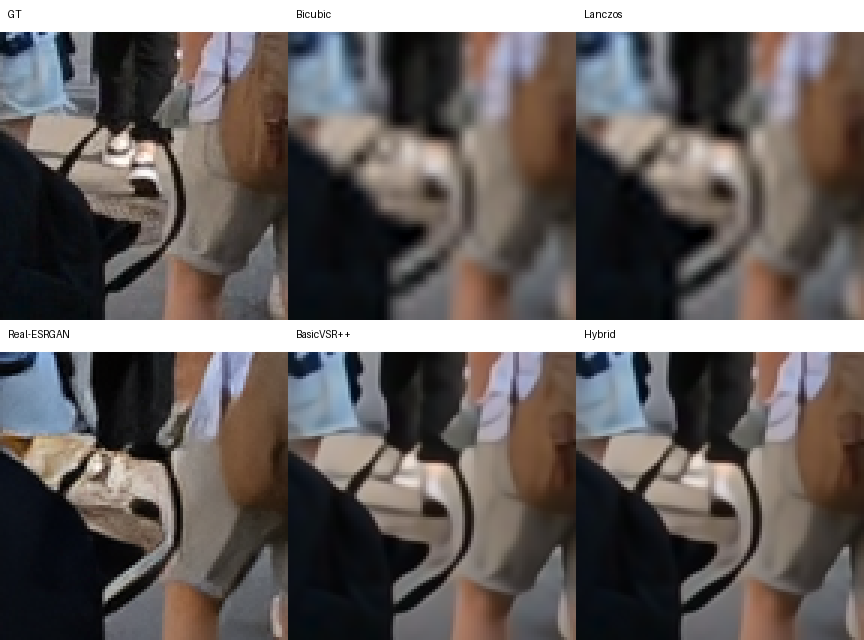
\includegraphics[width=\linewidth]{reds000_zoom_grid.png}
  \caption{Zoom-in patch comparison on REDS validation. The patch view highlights local edge and texture behavior across methods.}
  \label{fig:zoom}
\end{figure}

\subsection{Qualitative Analysis}
The qualitative results are consistent with the quantitative trends. Bicubic and Lanczos are visually stable but blurry, especially in fine textures. SRCNN does not consistently improve over interpolation, reflecting the limitation of shallow CNNs and lightweight training. Temporal averaging can smooth noise but fails under motion because frames are not aligned. Real-ESRGAN produces sharper local details, but these details may not match GT and can vary frame by frame. BasicVSR++ provides the most faithful reconstruction by exploiting temporal propagation. The adaptive hybrid preserves most BasicVSR++ structure while adding limited perceptual enhancement in textured regions.

The zoom-in patches in Fig.~\ref{fig:zoom} further clarify the metric behavior. BasicVSR++ preserves object boundaries and background structure in a GT-aligned way, which explains its high PSNR and SSIM. Real-ESRGAN often increases apparent sharpness but may alter exact textures, which explains the gap between perceptual and pixel metrics. The hybrid inherits the BasicVSR++ layout and only partially admits Real-ESRGAN details, so its distortion scores remain close to BasicVSR++.

The additional FID and tLPIPS plots in Fig.~\ref{fig:fidtlpips} provide another view of the trade-off. Real-ESRGAN has much stronger perceptual scores than the classical methods, but it is not the best pixel-accurate reconstruction. Temporal averaging has poor tLPIPS because unaligned averaging changes motion patterns. BasicVSR++ and the hybrid keep temporal behavior much closer to GT than the naive temporal baseline, which supports the project goal of maintaining temporal consistency instead of only sharpening individual frames.

\section{Discussion}
The experiments show that VSR quality depends on both temporal modeling and the chosen objective. PSNR/SSIM favor GT-aligned reconstructions, where BasicVSR++ is strongest. Perceptual metrics favor visually sharper outputs, where Real-ESRGAN becomes more competitive. The adaptive hybrid demonstrates that a simple pixel-wise mask can combine these behaviors without retraining. However, it does not fully solve temporal consistency. The current tLPIPS is warpless and does not explicitly compensate for motion; future work could include optical-flow-aligned temporal metrics.

The full REDS benchmark strengthens the evidence beyond the mandatory sample data. Nevertheless, computational cost limited the full benchmark to BasicVSR++ rather than both BasicVSR and BasicVSR++. We consider this acceptable because BasicVSR++ is the stronger representative and BasicVSR was already reproduced on the sample datasets.

\section{Conclusion}
We completed all three required parts of the VSR project. Part~1 established classical and shallow CNN baselines. Part~2 reproduced pretrained Real-ESRGAN, BasicVSR, and BasicVSR++ pipelines. Part~3 introduced an adaptive hybrid refinement that fuses BasicVSR++ and Real-ESRGAN to explore the perception-distortion trade-off. Quantitative and qualitative results on mandatory data and full REDS validation show that BasicVSR++ is the best distortion-oriented method, Real-ESRGAN is useful for perceptual detail, and the adaptive hybrid provides a low-cost extension that stays close to BasicVSR++ while incorporating controlled perceptual enhancement.

\section*{Limitations and Future Work}
Our SRCNN baseline is shallow and uses limited weights, so it does not fully represent modern image SR. The temporal averaging baseline has no motion compensation and is mainly a diagnostic failure case. Real-ESRGAN is frame-independent and may flicker. The adaptive hybrid uses hand-crafted masks rather than learned uncertainty estimates. Future work could train a lightweight temporal fusion network, add optical-flow-aligned tLPIPS, evaluate additional benchmarks such as Vimeo-90K, and explore generative priors such as diffusion, ControlNet, or flow matching with explicit temporal constraints.

{
    \small
    \bibliographystyle{ieeenat_fullname}
    \bibliography{main}
}

\end{document}
